\documentclass[conference]{IEEEtran}
\IEEEoverridecommandlockouts
\usepackage{cite}
\usepackage{amsmath,amssymb,amsfonts}
\usepackage{algorithmic}
\usepackage{graphicx}
\usepackage{textcomp}
\usepackage{xcolor}
\usepackage{ctex}
\usepackage{booktabs}

\def\BibTeX{{\rm B\kern-.05em{\sc i\kern-.025em b}\kern-.08em
    T\kern-.1667em\lower.7ex\hbox{E}\kern-.125emX}}

\begin{document}

\title{基于500m网格的深圳市南山区多源数据融合与空间分析}

\author{\IEEEauthorblockN{宋阳霆}
\IEEEauthorblockA{\textit{城乡规划专业} \\
\textit{哈尔滨工业大学（深圳）}\\
深圳，中国 \\
学号：2023315113 }
}

\maketitle

\begin{abstract}
本研究以深圳市南山区为研究区域，基于500米$\times$500米网格单元，融合POI兴趣点、道路网络、建筑轮廓、DEM高程和遥感影像等多源数据，计算功能混合度、POI密度、路网密度、容积率、平均高程和平均绿化度(NDVI)等6项空间指标，分析其空间分布格局及相互关系。数据坐标统一为CGCS2000 3度带投影坐标系(中央经线114$^\circ$E, EPSG:4527)。POI数据经GCJ-02坐标纠偏(偏移量约540m经度/335m纬度)后转为WGS84再投影。研究区共划分761个网格单元，其中552个网格含有POI数据。
\end{abstract}

\begin{IEEEkeywords}
GIS；多源数据融合；功能混合度；空间分析；CGCS2000；南山区
\end{IEEEkeywords}

\section{研究概述}

本研究以深圳市南山区为研究区域，基于500米$\times$500米网格单元，融合POI兴趣点、道路网络、建筑轮廓、DEM高程和遥感影像等多源数据，计算功能混合度、POI密度、路网密度、容积率、平均高程和平均绿化度(NDVI)等6项空间指标，分析其空间分布格局及相互关系。

数据坐标统一为CGCS2000 3度带投影坐标系(中央经线114$^\circ$E, EPSG:4527)。POI数据经GCJ-02坐标纠偏(偏移量约540m经度/335m纬度)后转为WGS84再投影。研究区共划分761个网格单元，其中552个网格含有POI数据。

\section{数据与方法}

\subsection{数据来源与预处理}

POI数据：NSPOI.shp，84279个兴趣点，含Type分类字段(10大类)。原始坐标为GCJ-02火星坐标系(EPSG:3857)，经纠偏后转为WGS84(EPSG:4326)再投影至CGCS2000。纠偏后网格内POI共83544个，损失率0.9\%。

道路数据：南山区道路中心线.shp，33356条道路。投影后计算道路长度。

建筑数据：深圳建筑轮廓数据，全市144781栋，南山区内裁剪得24795栋。Floor字段清洗($\leq 0$设为1)，投影后计算底面积和建筑面积。

DEM数据：nanshanDEM.img，原始UTM Zone 49N(EPSG:32649)，分辨率约30m，逐网格裁剪统计平均高程。

遥感影像：NSRS.tif，7波段Landsat影像(EPSG:32649)，用Band3(Red)和Band4(NIR)计算NDVI=(NIR-Red)/(NIR+Red)。

行政边界：nanshanDomain.shp，南山区行政边界，原始EPSG:3857。

\subsection{指标计算方法}

功能混合度采用信息熵标准化公式：
\begin{equation}
H = -\frac{\sum_{i=1}^{N} P_i \ln P_i}{\ln N}
\end{equation}
其中$N=10$为POI类型数，$P_i$为第$i$类占比。两种占比方式：绝对数量占比$P_i = n_i / \sum_j n_j$；积聚程度占比$P_i = \sqrt{n_i/A} / \sum_j \sqrt{n_j/A}$，$A=250000$\,m$^2$。

其他指标：POI密度=网格内POI总数/0.25\,km$^2$；路网密度=裁剪后道路总长(km)/0.25\,km$^2$；容积率=建筑总面积(底面积$\times$楼层数之和)/网格面积(250000\,m$^2$)；平均高程和NDVI由栅格逐网格裁剪统计获得。

\section{空间分布格局分析}

\subsection{功能混合度}

绝对数量混合度均值为0.571，最大值0.926；积聚程度混合度均值为0.646，最大值0.980。高混合度区域集中在中西部建成区(南山街道、粤海街道)，POI类型多样且分布均匀。低混合度区域分布在北部山区(塘朗山-大沙河生态廊道)和南部沿海区域，POI类型单一。积聚程度混合度普遍高于绝对数量混合度，差异在商业密集区更明显，说明积聚校正能更好反映小类别的存在感。图~\ref{fig:mixity}对比了两种混合度的空间分布。

\begin{figure}[htbp]
\centerline{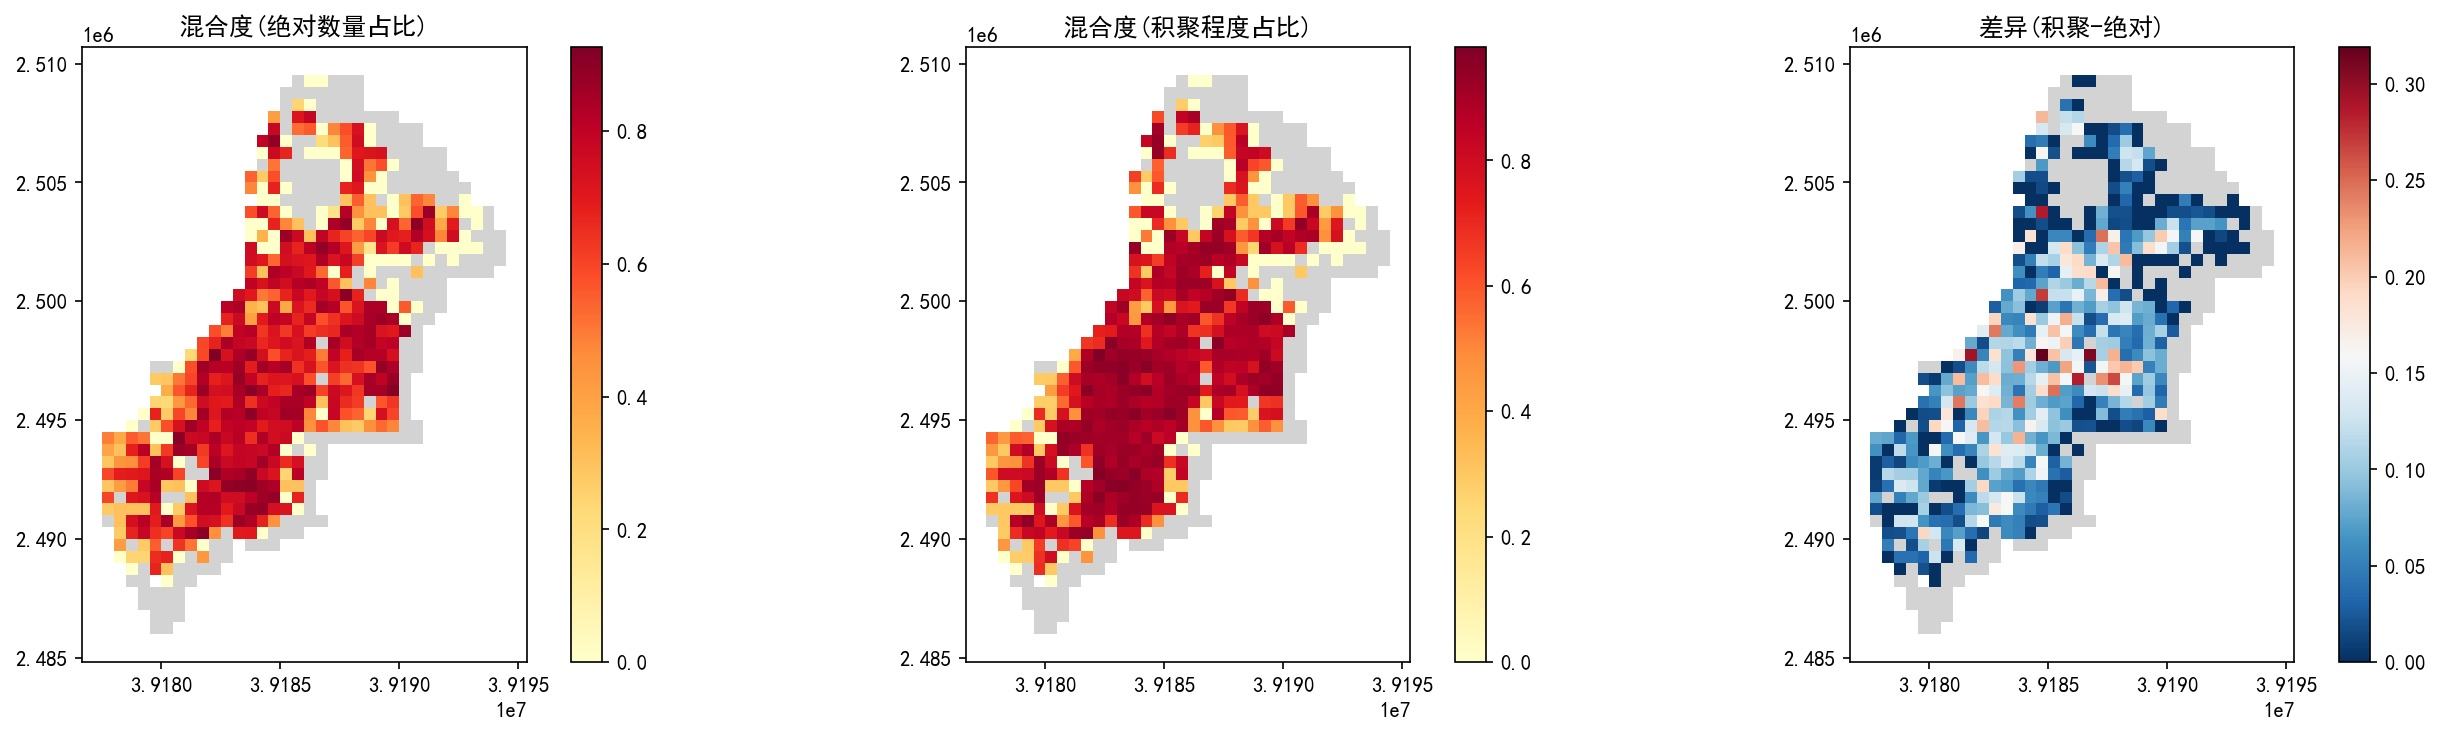
\includegraphics[width=\columnwidth]{fig2.jpg}}
\caption{绝对数量混合度与积聚程度混合度对比}
\label{fig:mixity}
\end{figure}

\subsection{POI密度}

POI密度均值为607.5个/km$^2$，中位数为110.0个/km$^2$，呈明显右偏分布。高密度区域集中在后海-深圳湾片区和科技园片区，POI密度最高达10628个/km$^2$；北部山区和南部大南山区域POI密度极低。空间分布呈现"西密东疏、南密北疏"的格局(图~\ref{fig:poi})。

\begin{figure}[htbp]
\centerline{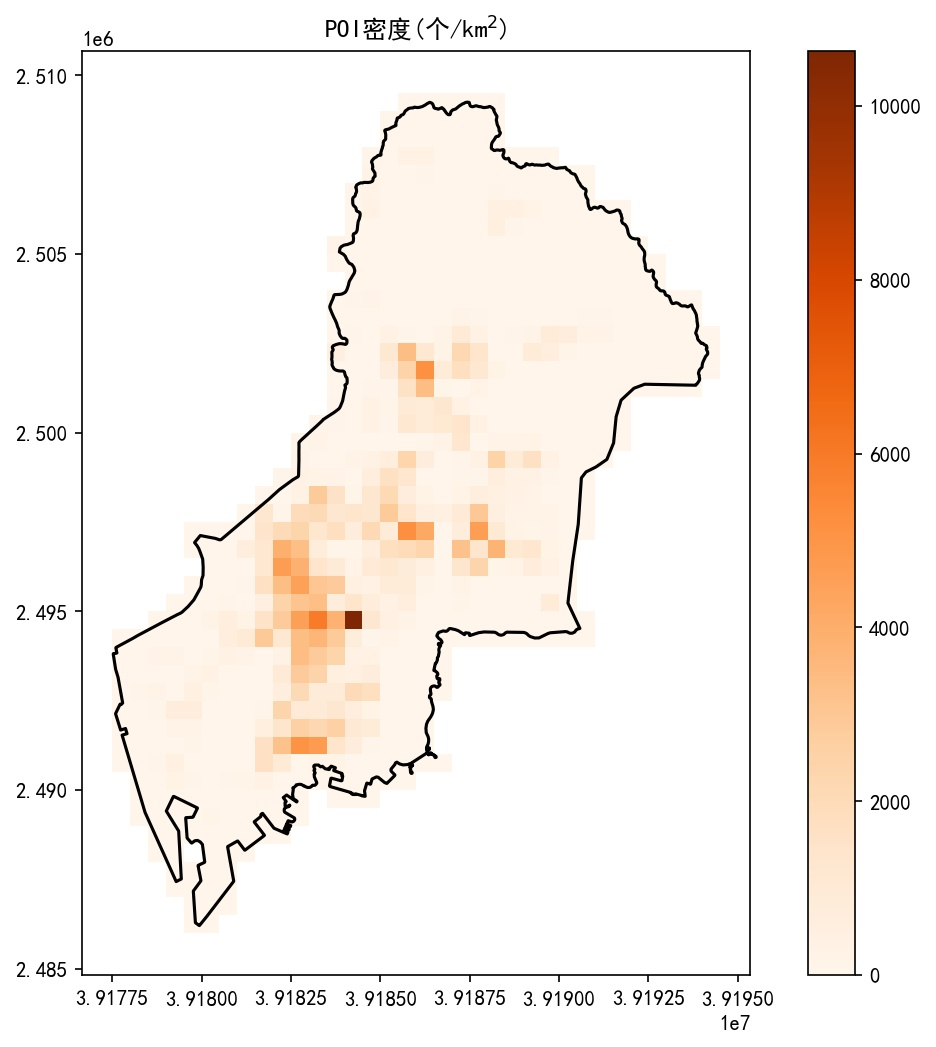
\includegraphics[width=\columnwidth]{fig3.jpg}}
\caption{POI密度空间分布}
\label{fig:poi}
\end{figure}

\subsection{路网密度}

路网密度均值为17.79\,km/km$^2$，最大值44.13\,km/km$^2$。高路网密度区域与城市核心区高度重合，前海-后海片区路网密度最高，反映该区域道路网络发达。北部山区路网密度较低，受地形限制道路建设较少(图~\ref{fig:road})。

\begin{figure}[htbp]
\centerline{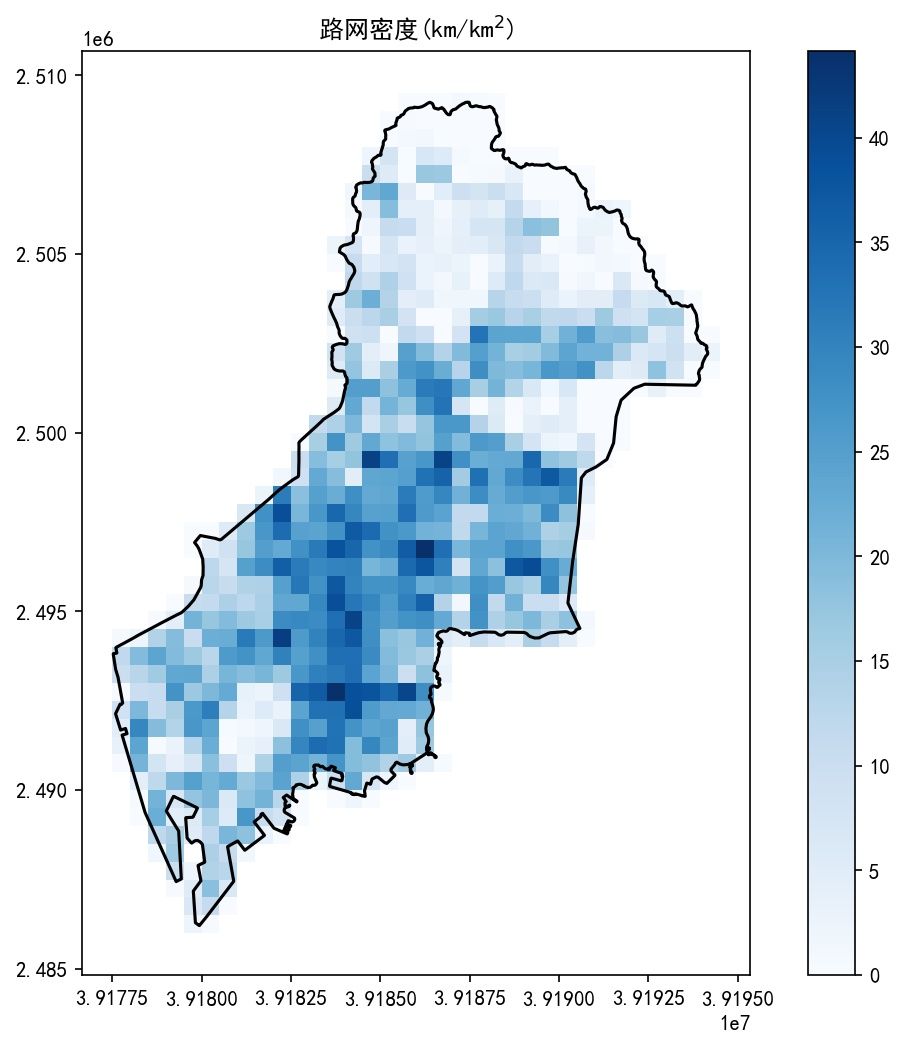
\includegraphics[width=\columnwidth]{fig4.jpg}}
\caption{路网密度空间分布}
\label{fig:road}
\end{figure}

\subsection{容积率}

容积率均值为0.548，中位数0.225，呈右偏分布。高容积率区域集中在后海CBD和科技园高层建筑密集区，容积率最高达4.474。大部分区域容积率低于1.0，反映南山区整体开发强度适中但局部高度集中(图~\ref{fig:far})。

\begin{figure}[htbp]
\centerline{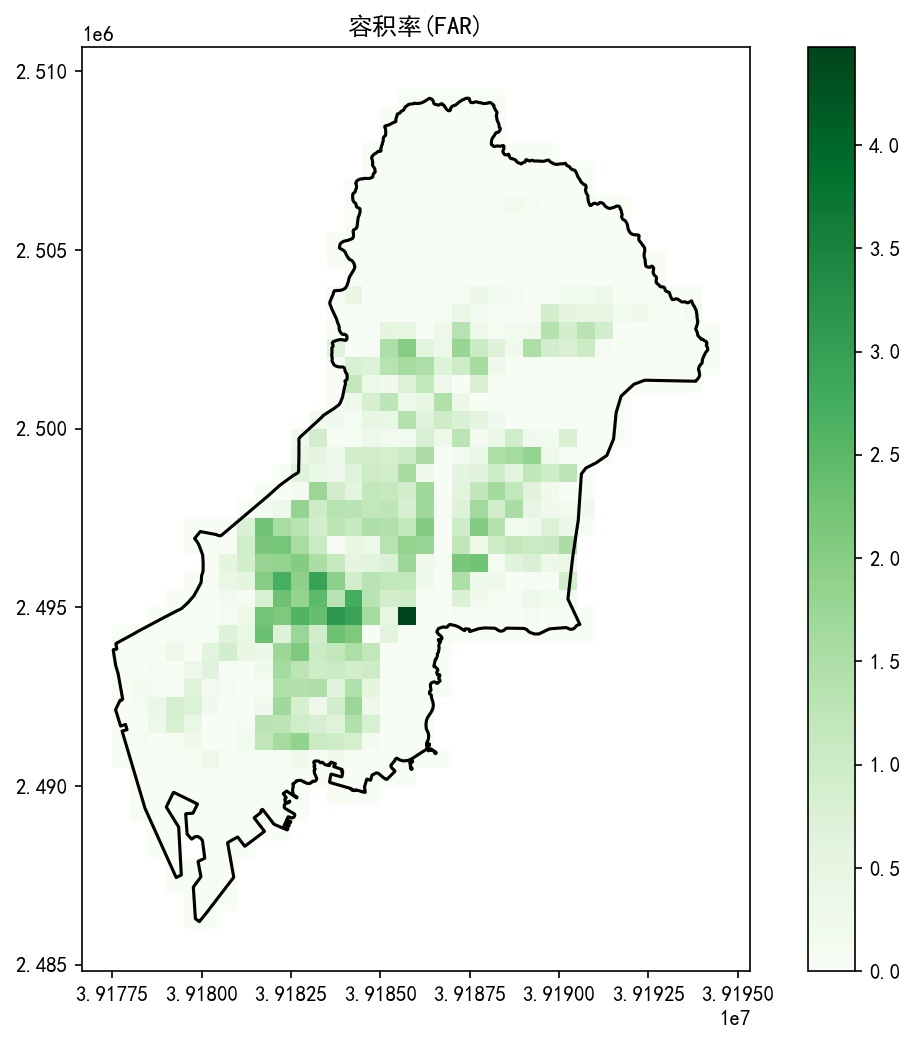
\includegraphics[width=\columnwidth]{fig5.jpg}}
\caption{容积率空间分布}
\label{fig:far}
\end{figure}

\subsection{高程与绿化度}

平均高程均值为28.5\,m，最大值342.3\,m；NDVI均值为0.081，最大值0.346。高程与NDVI呈显著正相关($r=0.633$)，山区植被覆盖度高。高程与所有城市指标(混合度、POI密度、路网密度、容积率)均呈负相关，反映地形对城市开发的限制作用。图~\ref{fig:spatial}展示了六项指标的综合空间分布。

\begin{figure}[htbp]
\centerline{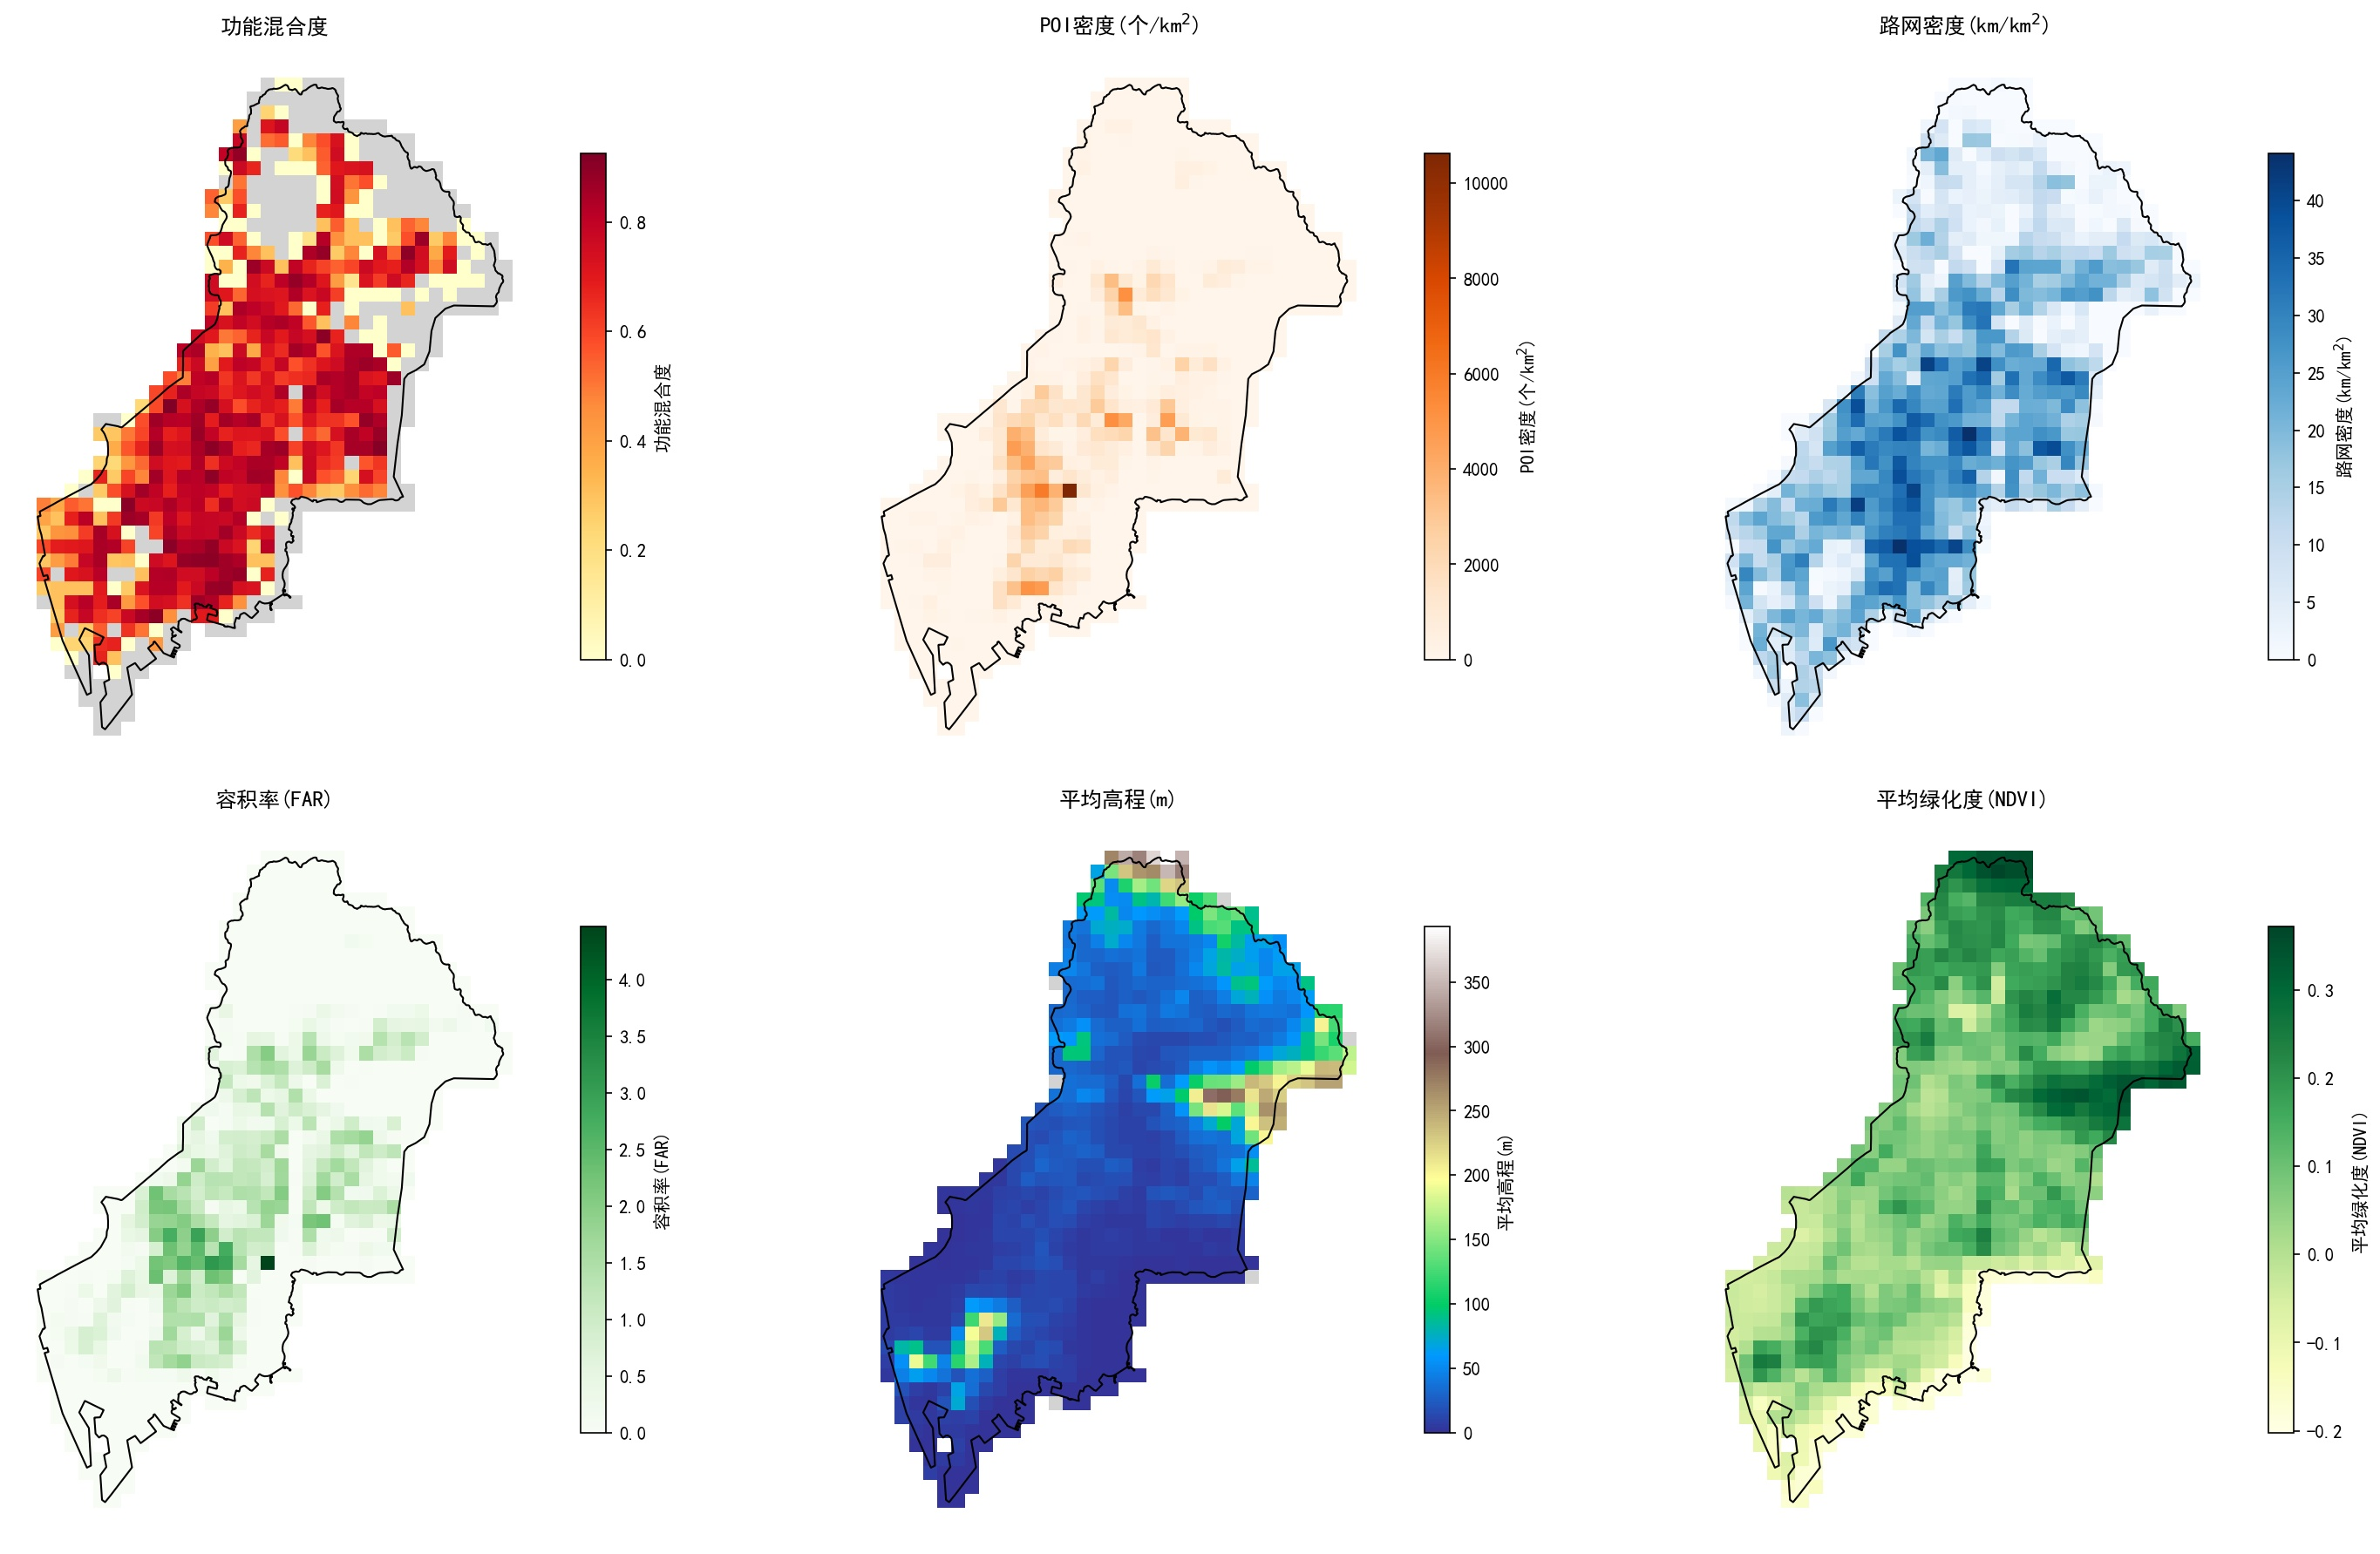
\includegraphics[width=\columnwidth]{fig1.jpg}}
\caption{南山区六项指标空间分布}
\label{fig:spatial}
\end{figure}

\section{指标关系分析}

6项指标的相关系数矩阵如图~\ref{fig:corr}所示，散点图矩阵如图~\ref{fig:scatter}所示。主要发现：POI密度与容积率正相关最强($r=0.720$)，商业密集区建筑开发强度高；功能混合度与容积率正相关($r=0.518$)，多功能混合区域往往开发强度较高；功能混合度与路网密度正相关($r=0.460$)，道路网络支撑了功能多样性；高程与路网密度负相关($r=-0.379$)，地形制约道路建设；高程与NDVI正相关($r=0.633$)，山区绿化覆盖度高；NDVI与城市指标均呈弱负相关，城市开发与植被覆盖存在此消彼长关系。

\begin{figure}[htbp]
\centerline{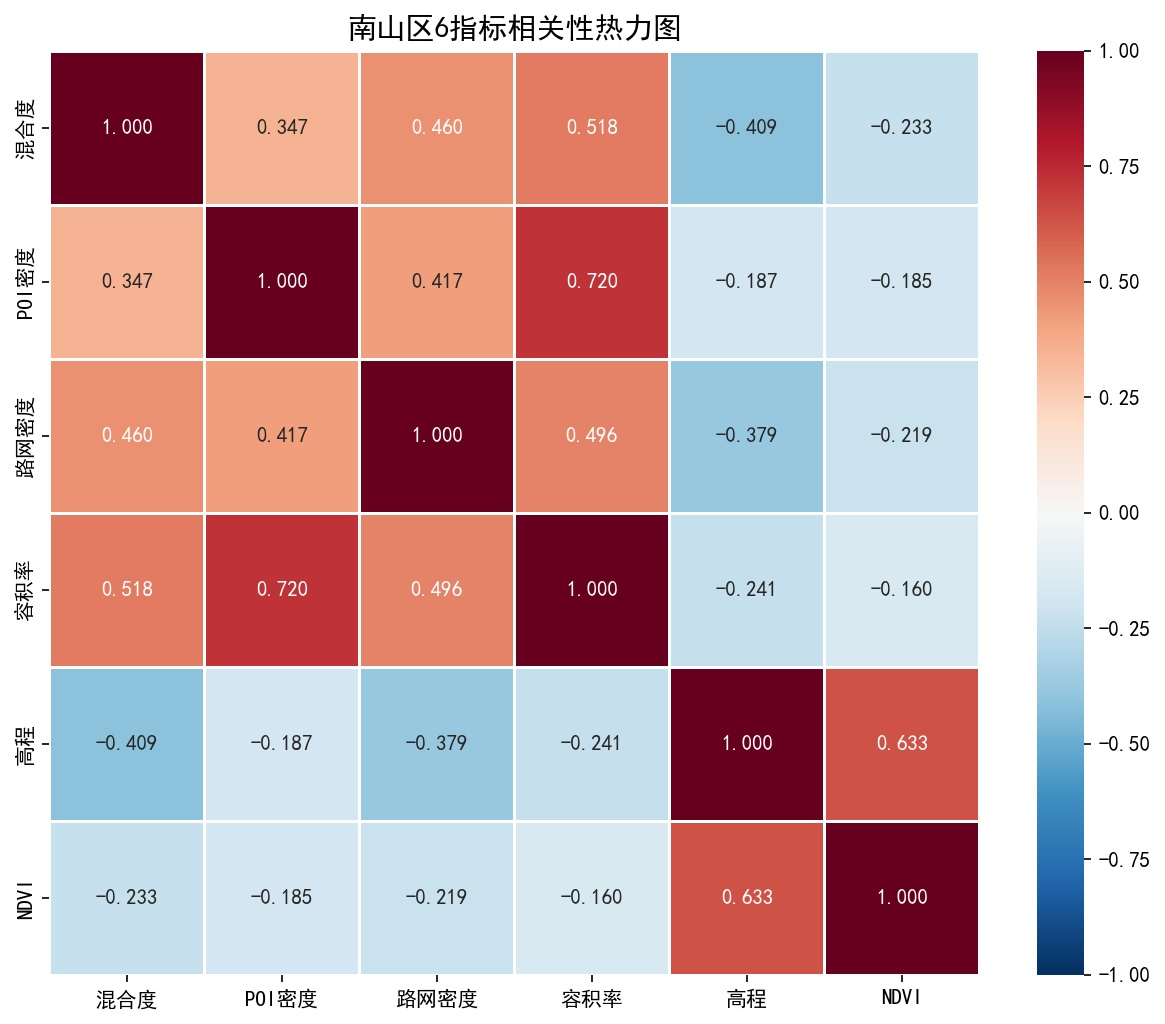
\includegraphics[width=\columnwidth]{fig6.jpg}}
\caption{六指标相关系数热力图}
\label{fig:corr}
\end{figure}

\begin{figure}[htbp]
\centerline{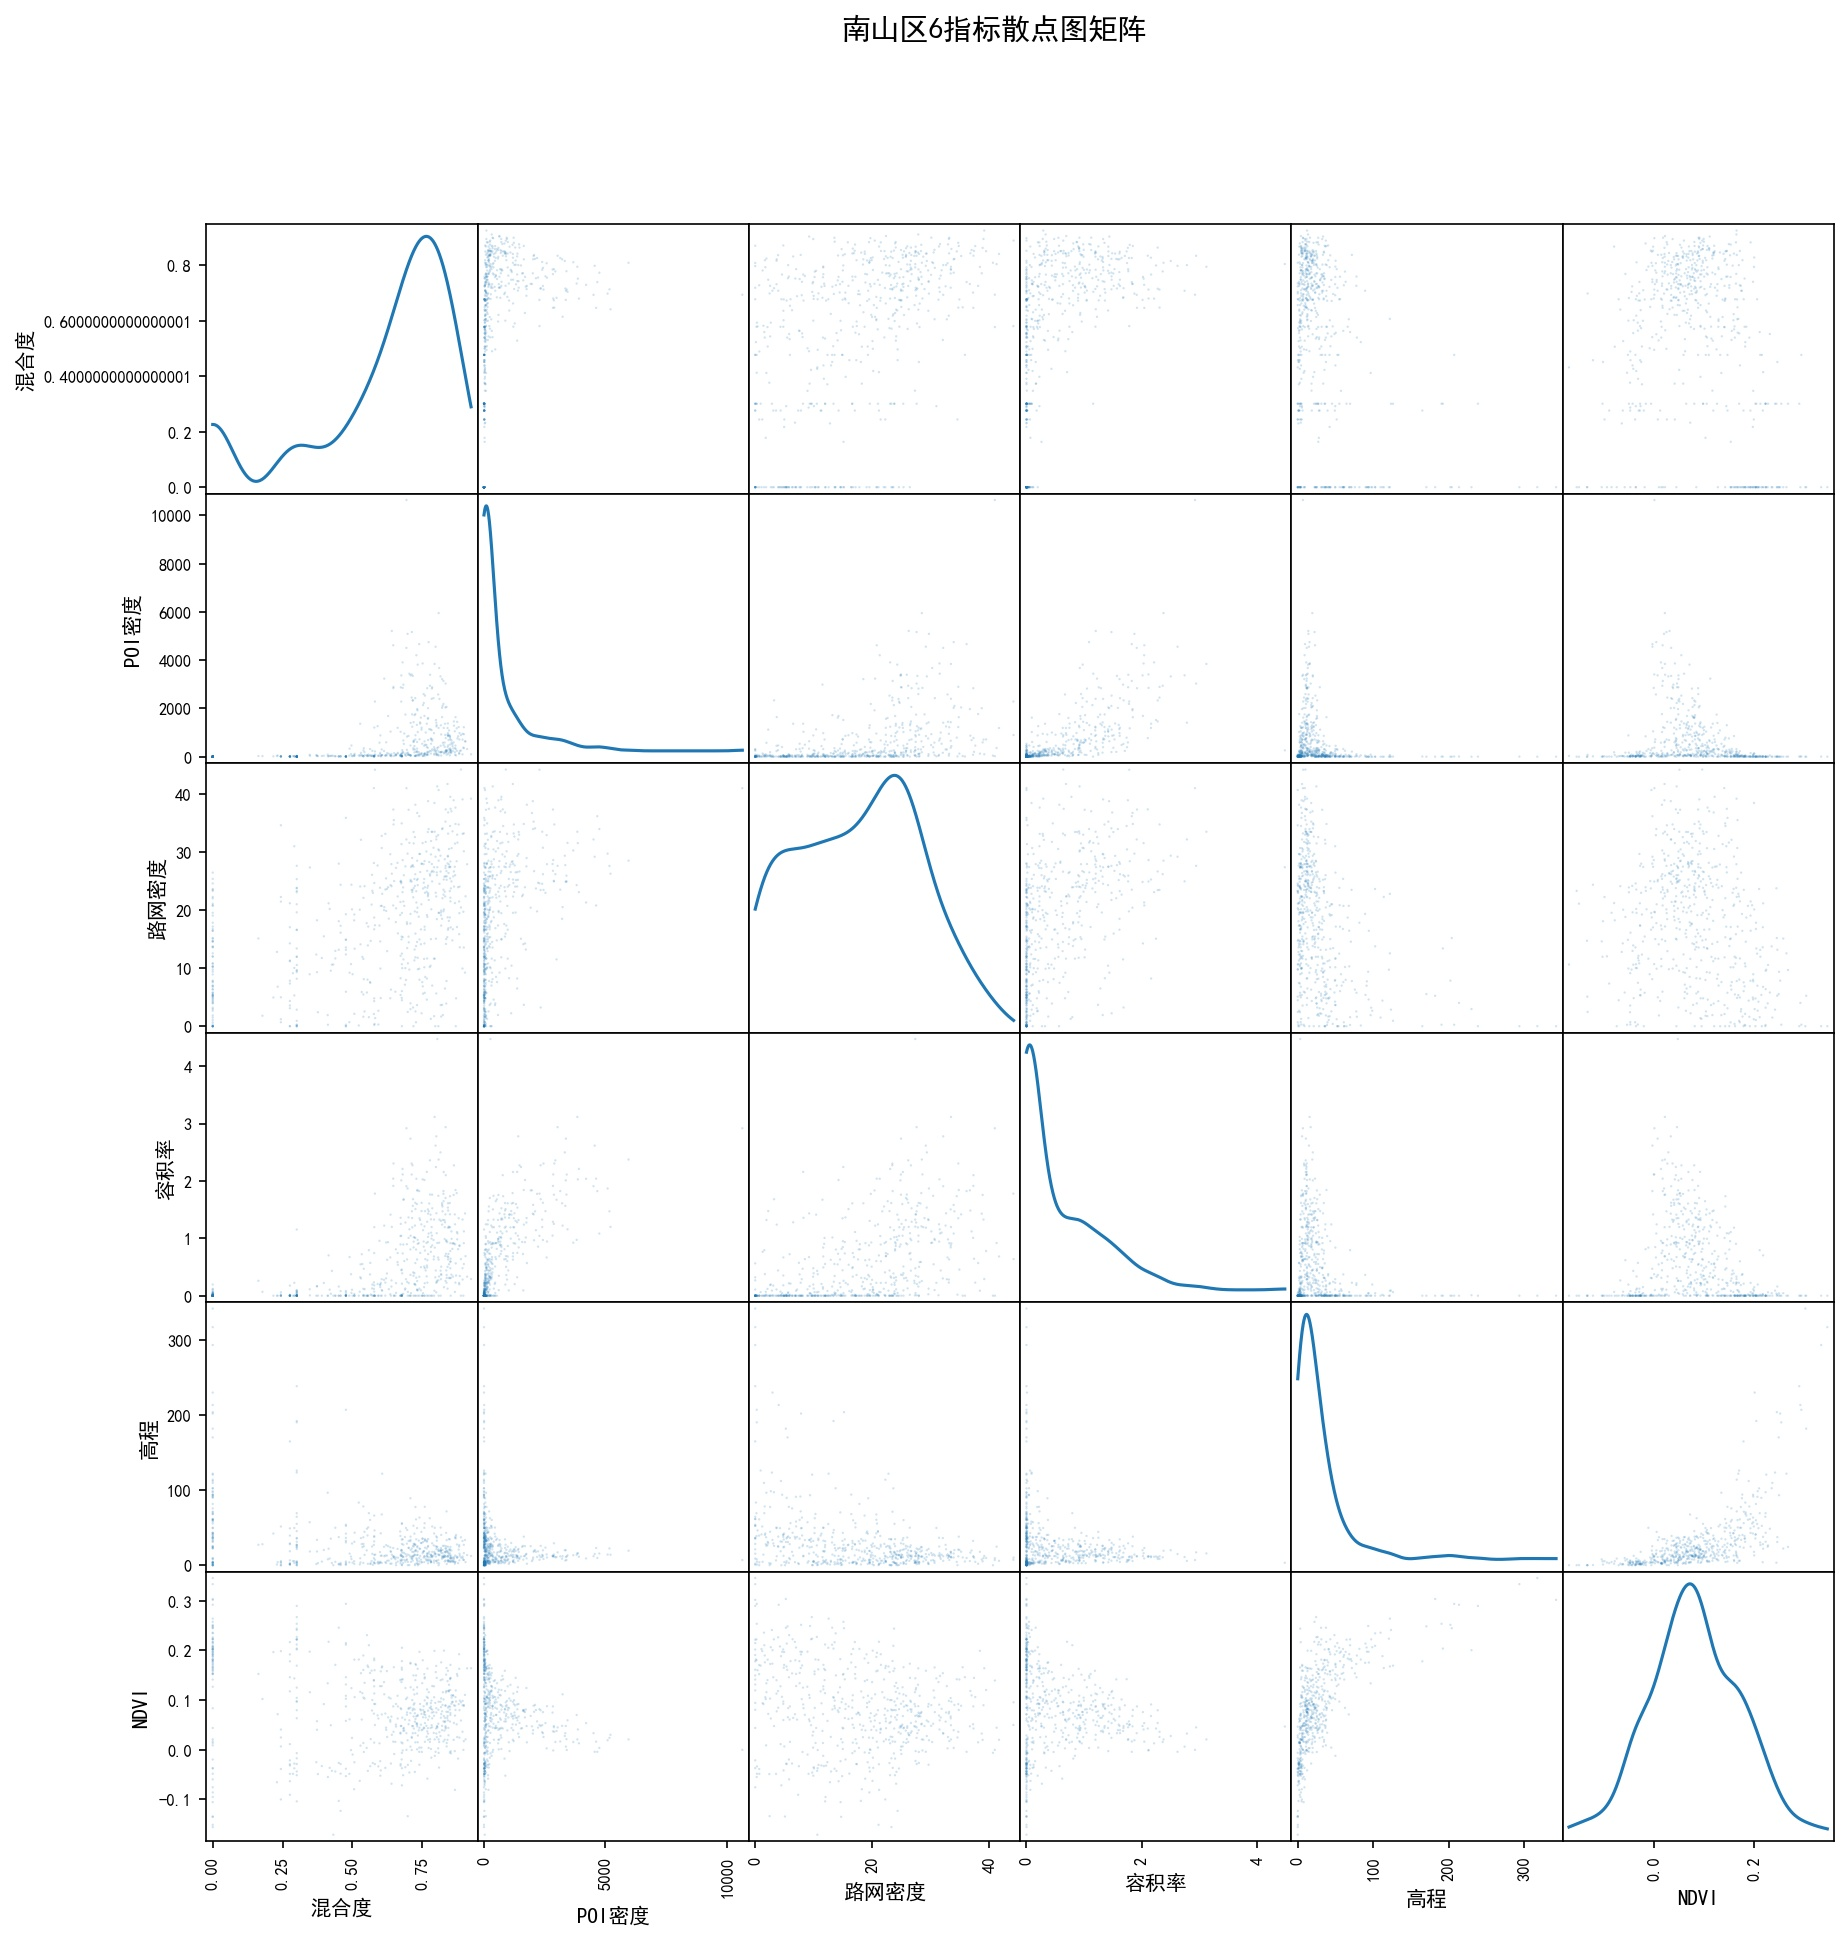
\includegraphics[width=\columnwidth]{fig7.jpg}}
\caption{六指标散点图矩阵}
\label{fig:scatter}
\end{figure}

\section{结论}

南山区城市空间呈现"核心-边缘"分异格局：中西部平原建成区功能混合度高、POI密度大、路网密集、容积率高；北部山区和南部大南山区域则高程高、绿化度好但城市指标低。地形是制约城市开发的关键因素，高程与所有城市指标负相关、与NDVI正相关。POI密度与容积率高度正相关($r=0.720$)，表明商业活力与建筑开发强度空间耦合。积聚程度混合度相比绝对数量混合度更能体现小类别的贡献，在商业密集区差异尤为明显。

\begin{thebibliography}{00}
\bibitem{b1} 龙瀛, 周麟, ``基于POI的城市功能混合度测度与空间格局分析,'' \textit{城市规划学刊}, no. 5, pp. 40--47, 2019.
\bibitem{b2} 李刚, ``GCJ-02坐标系偏移分析与校正方法,'' \textit{测绘科学技术学报}, vol. 38, no. 3, pp. 245--251, 2021.
\bibitem{b3} K. Frank and M. C. J. Bervoets, ``Functional mixity and urban vitality: Measuring diversity with entropy indices,'' \textit{Urban Stud.}, vol. 59, no. 4, pp. 812--830, 2022.
\bibitem{b4} 池娇, 焦利民, 董婷, 等, ``基于POI数据的城市功能区识别与空间结构分析,'' \textit{地理与地理信息科学}, vol. 35, no. 1, pp. 56--62, 2019.
\bibitem{b5} M. Batty, \textit{Cities and Complexity: Understanding Cities with Cellular Automata, Agent-Based Models, and Fractals}, MIT Press, 2007.
\bibitem{b6} S. Fotheringham and D. Wong, ``The modifiable areal unit problem in multivariate statistical analysis,'' \textit{Environ. Plan. A}, vol. 23, no. 7, pp. 1025--1044, 1991.
\end{thebibliography}

\end{document}
